\documentclass{article}
\usepackage{graphicx}
\usepackage{float}
\usepackage{amsmath}
\begin{document}
	\title{Diari Joc Quàntic}
	\author{Adrià Bravo Vidal}
	\date{24/04/20}
	\maketitle	
	
\renewcommand{\abstractname}{Introducció}	
\begin{abstract}
	Desenvolupament de un joc per la divulgació quàntica. Avanços i sobretot, problemes en el camí a construir el nombrat joc.
\end{abstract}
\tableofcontents

\section{Progrmació Crank-Nicolson}

L'objectiu es programar la evolució d'un paquet gaussià dins una caixa 2D amb potencial infinit als cantons. Per fer-ho, cal resoldre la equació de 
Schrodinger:

\begin{equation}
i\hbar\frac{\partial}{\partial t}\psi=H\psi
\end{equation}

En aquest cas, ja que operarem en l'espai de posicions, podem expresar l'operador H així:

\begin{equation}
H=-\frac{\hbar^2}{2m}(\frac{\partial^2}{\partial x^2}+\frac{\partial^2}{\partial y^2}) + V(x,y)
\end{equation}

Sigui una caixa quadrada 2D amb dimensions a=2L, el potèncial que aplicarem serà:

\begin{equation}
V(x,y) = \left\{
\begin{array}{lr}
\infty & : |x|\quad and\quad |y| > L\\
V_i(x,y) & : |x|\quad or\quad |y|< L 
\end{array}
\right.
\end{equation}

On \(V_i\) és el potencial que volguem aplicar a l'interior de la caixa. El mètode que seguirem per resoldre la equació sera el mètode ADI (alternating
direction implicit metohd). Aquest es basa en la utilització del mètode de Crank-Nicolson per resoldre l'equació (1). Primer de tot, comprovarem com funciona el mètode de Crank-Nicolson en 1D i posteriorment, aplicarem el mètode ADI en si.

\subsection{Crank-Nicolson en 1D}

El mètode de Crank-Nicolson és un mètode implicit amb el que s'obté estabilitat incondicional per cada dt i dx escollits. Ofereix una conservació de la norma total. No obstant, caldrà escollir dt i dx més o menys petits per raons de coherència física (dt i dx massa grans no resoldran be el problema ja que el simplificaran massa).

L'algoritme i les equacions a utiltzar es poden obtenir aplicant una derivada de temps de \(0.5\Delta t \) desde l'estat actual \(t\) fins \(t+0.5\Delta t\) i un altre igual pero retrocedint desde \(t+\Delta t\) fins \(t+0.5\Delta t\). Així obtenim la següent relació:
			
\begin{equation}
(1+i\frac{\Delta t}{2})Hpsi(x,t+\Delta t)=(1-i\frac{\Delta t}{2})Hpsi(x,t)
\end{equation}
	
Ara, discretitzarem la nostra recta en \(Nx=2L/dx\) troçets, i aplicarem el següent criteri: \(x=-L+i*dx\), on \(i=0,...,Nx\). Fem el mateix pel temps, i obtenim que \(Nt=\frac{t_b-t_a}{dt}\) on t=tb+k*dt. Utilitzant la discretització de la segona derivada en x i ordenant els termes de l'equació anterior, obtindrem:


\begin{align}
&\psi_i^{k+1}[1+\frac{i\Delta t}{2\hbar}(V_i+\frac{\hbar^2}{m\Delta x ^2})]-\frac{\hbar\Delta t}{4m \Delta x^2}(\psi_{i+1}^{k+1}+\psi_{i-i}^{k+1})\\
&=\psi_i^{k}[1-\frac{i\Delta t}{2\hbar}(V_i+\frac{\hbar^2}{m\Delta x ^2})]+\frac{\hbar\Delta t}{4m \Delta x^2}(\psi_{i+1}^{k}+\psi_{i-i}^{k})
\end{align}


Estudiant aquesta equació, ens adonem que obeeixen un sistema on tenim Nx incognites (és a dir, \(\psi_i^{k+1}\) on i=1,...Nx) i Nx equacions (una (5) per cada i). Per tant, aquest sitema té solució. A més, comporta l'adventatja de ser tridiagonal. Es a dir, si expresem el sistema en forma matriarcal:

\begin{equation}
A\psi^{k+1}=B\psi^{k}
\end{equation}   

Tindrem que la matriu A del sistema és tridiagonal. Aprofitant aquest fet, el sistema és pot resoldre rapiadment gràcies a un algoritme específic per aquest tipus de matrius que necesita només Nx operacions. Aixi, donat un vector \(psi^0\) inicial i coneguent el potèncial \(V(x,y)\) en el que es troba, podem fàcilment conéixer \(psi^k\) en qualsevol instant de temps. 

\subsection{Crank-Nicolson en 2D: ADI}

Recuperem ara, el problema inicial en 2D. L'aplicació directe del mèotde de Crank-Nicolson a l'equació de Schrödinger 2D funciona però la matriu resultant és tan ample que els temps de computació s'allarguen massa. El que es fa, llavors, és el que s'anomena alternating direction implicit metodh (ADI). En aquests casos el que es fa es dividir el numero de equacions entre dos. Una, pren la derivada de X implicitament (és a dir, pren la derivada de x en\(k+\frac{1}{2}\)) i la de Y explicitament (és a dir, en \(k\)) i s'obté \(psi^{k+\frac{1}{2}}\). La pròxima, pren \(psi^{k+\frac{1}{2}}\), fa la derivada de Y implicitament i la de X explicitament i avança fins \(k+1\), obtenint \(psi^{k+1}\). Això completaria un pas del mètode ADI. 

Pel problema en 2D discretitzarem l'espai i el temps de la mateixa manera que en el cas 1D. Donada una caixa de a=2L de costat, podem definir un dx que per simplicitat igualarem a dy, que ens donara un mallat Nx, Ny. En quant al temps, procedim igual:

\begin{equation}
Nx,Ny=\frac{2L}{dx}, \quad Nt=\frac{t_b-t_a}{dt}
\end{equation}

Un cop tenim la nostra malla discretitzada, podem discretitzar tambe la nostre funció de ona tal quee així:

\begin{equation}
\psi(x_i,y_j)=psi_{i,j}, \quad x_i=-L+idx,y_j=-L+jdx
\end{equation}

Si ara desenvolupem el procediment descrit anteriorment i definim \(r=\frac{\Delta t \hbar}{4\Delta x^2 m}\), obtindrem una equació com aquesta que descriu la primera iteració del mètode ADI:

\begin{align}
&\psi_{i,j}^{k+1/2}[1+\frac{i\Delta t}{4\hbar}V_i+2r]-r(\psi_{i+1,,j}^{k+1}+\psi_{i-1,j}^{k+1}) = \\
&\psi_{i,j}^{k}[1-(\frac{i\Delta t}{2\hbar}V_i+r)]+r(\psi_{i,j+1}^{k}+\psi_{i,j-1}^{k})
\end{align}

La equació corresponant a la segona iteració es pot obtenir intercanviant i per j i fent el canvi \(k=k+1/2 \). Estudiem la equació de la primera iteració. Donat un columna j inicial, la part esquerra de la equació només itera sobre aquesta columna. Per tant, estem iterant sobre el vector corresponent a la columna j. Això implica que, donada la forma idèntica amb la equació pel cas 1D, tornem a tenir un sistema que es pot expressar així: \(A\psi_{:,j}^(k+1/2)=B\). Aquest cop, però, B serà més elaborada, ja que tindra en compte el vector columna j, j+1 i j-1. El cas per i inicial fixat al mebre esquerre és analog al que s'acaba d'explicar. Aquesta és la idea que hi ha darrera l'elaboració d'un mètode ADI. 

\section{Convergència en l'aplicació del mètode}

Un cop programat el mètode ADI cal testejar-lo. Mentiria si digués que no ho he fet ja un cop, pensant que l'havia programat bé. De fet, parlant d'aquest últim cas, el vaig testejar força: coservació de la norma, de la energia... Però vaig arribar al potèncial harmònic i em  vaig adonar de que hi havia d'haver algún error conceptual amb el codi (després de deixar-me els ulls buscant algún error.) Efectivament, existia. No havia entés bé el mètode ADI i m'havia patillat una cosa que tot i ser semblant, no era un mètode coherent. No obstant, ha estat ràpid tornar a generar totes les gràfiques ja que ho tinc tot molt automitzat.

Primer de tot, cal escollir tot un seguït de paramètres,i el paquet amb el que jugarem. Treballarem amb \(\hbar=1,m=1\)

\subsection{Elecció d'un paquet i un discretitzat}

Primer de tot, cal pensar que el paquet d'ones més simple amb el que podem treballar és un paquet gaussià, ja que és el que satura les relacions de incertesa (inicialment):

\begin{equation}
\psi(x,y)=\frac{1}{\sqrt{2\pi\sigma^2}}e^{-\frac{1}{4\sigma^2} (x^2+y^2)+\frac{i}{h} (p_{ox} x +p_{oy} y)}	
\end{equation}

En aquesta equació, suposem \(\sigma_x=\sigma_y=\sigma\). Escollirem, arbitarariament, una L=3 (d'acord amb les unitats descrites anteriorment). A partir d'aquí, un bon criteri per escollir un discretitzat adient és la energia del paquet. Hem de tenir en compte que aquest diferirà sempre de la teòrica i hom pot predir que quan més gran sigui el discretitzat, i per tant més imprecisa la solució de les equacions, més ens allunyarem de la energia total. Com calculem la energia cinètica i potèncial d'aquest paquet?

\subsubsection{Càclul de la energia}
Un bon indicador de quin discretitzat hem d'escollir és el càlcul de la energia del nostre paquet. Es pot calcular la energia cinètica d'un paquet gaussià sense moltes dificultats, i també es pot calcular la energia del paquet un cop discretitzat, és a dir, un calcul computacional que ens indiqui quina energia té el nostre paquet. La comparació d'aquests dos resultats ens donarà unas pautes per continuar. 

El càlcul de la energia en mecànica quàntica, com ja sabem, implica el càlcul del seu valor esperat. Així, tindrem que:

\begin{equation}
<H>=\int\int\psi*H\psi \mathrm{d}x^2
\end{equation}

Com bé sabem, l'operador H te la part cinètica diferenciada de la potencial, per tant d'aquí obtindrem la suma de dos integrals:

\begin{equation}
<V>=\int\int\psi*V\psi \mathrm{d}x^2
\end{equation}
\begin{equation}
<E_c>=\int\int\psi*-\frac{\hbar^2}{2m}(\frac{\partial^2}{\partial x^2}+\frac{\partial^2}{\partial y^2})\psi \mathrm{d}x^2
\end{equation}

Si apliquem el calcul de la energia cinètica pel nostre paquet gaussià en un espai infinit, obtindrem la següent equació:

\begin{equation}
E_c=\frac{\hbar^2}{2m}(p_{ox}^2+p_{oy}^2+\frac{1}{2\sigma^2})
\end{equation}

Ara voldriem comparar aquesta energia amb la que té el nostre paquet discretitzat amb un dx arbitari dins la caixa de a=2L. Aquí podriem preguntarnos si no és una comparació absurda, ja que els limits d'integració en un cas són infinits i en l' altres son \(x,y=\pm L\). Doncs bé, ja que el paquet es concentra molt, en aquest cas, en x=0 e y=0, és un aproximació prou bona comparar aquestes dues energias, tenint en compte que la del paquet discretitzat sempres serà menor que la teòrica ja que hi haurà elements que mai sumarem en el primer cas.

Per calcular la energia cinètica i potencial de un paquet discretitzat utilitzarem el següent algoritme


\textit{def Ham(psi,hbar,m,dx,Vvec):\\Matriu que ens calcula la energia total.\\Ec=np.zeros((np.shape(psi)),dtype=complex)\\Ep=np.zeros((np.shape(psi)))\\Nx=np.int(len(psi[0,:]))-1\\s=(1/2.)*(1./dx**2)\\for i in range(1,Nx):\\for j in range(1,Nx):\\Ec[i,j]=-s*(psi[i+1,j]+psi[i-1,j]+psi[i,j-1]+psi[i,j+1]-4*psi[i,j])\\Ec[i,j]=np.real(Ec[i,j]*np.conj(psi[i,j]))\\Ep[i,j]=psi[i,j]*np.conj(psi[i,j])*Vvec[i,j] }

Per calcular la energia cinètica utilitzem la formula de la segona derivada discretitzada en x i en y. Després, haurem de multiplicar pel psi[i,j]* al que hem aplicat aquella derivada i ens quedarem només amb la part real de l'assumpte, ja que l'energia és real. Aquest càlcul perd una mica d'informació ja que quan multipliquem psi[i,j]* per la derivada discretitzada, perdem la part imaginària i suposo que això no és del tot correcte. No obstant, funciona força bé. Posteriorment a la creacio de les matrius Ec i Ep, només haurem de aplicar-li una integració sobre tot x e y. 

Aplicant aquests dos calculs a diferents paquets de diferent \(p_{ox}\) i una \(\sigma^2=0.25\) obtenim figures com aquestes:

\begin{figure}[H]
	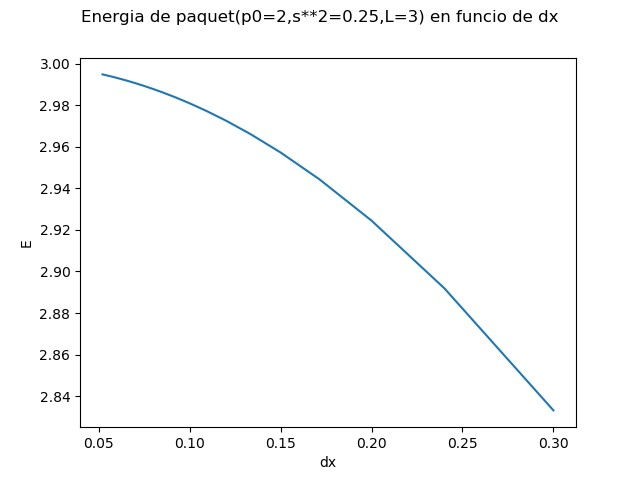
\includegraphics[width=\textwidth,height=7cm]{problemaenergia4.jpg}
	\caption{Energia cinètica de un paquet de \(p_{0x}=2,p_{oy}=0\)}
\end{figure}
\begin{figure}[H]
	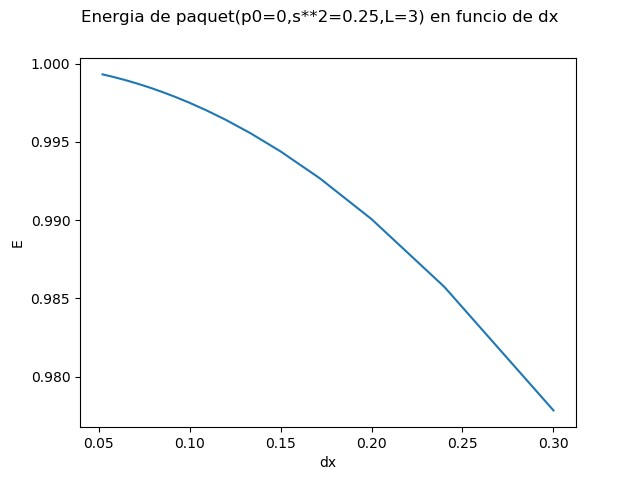
\includegraphics[width=\textwidth,height=7cm]{problemaenergia5.jpg}
	\caption{Energia cinètica de un paquet de \(p_{0x}=0,p_{oy}=0\)}
\end{figure}
\begin{figure}[H]
	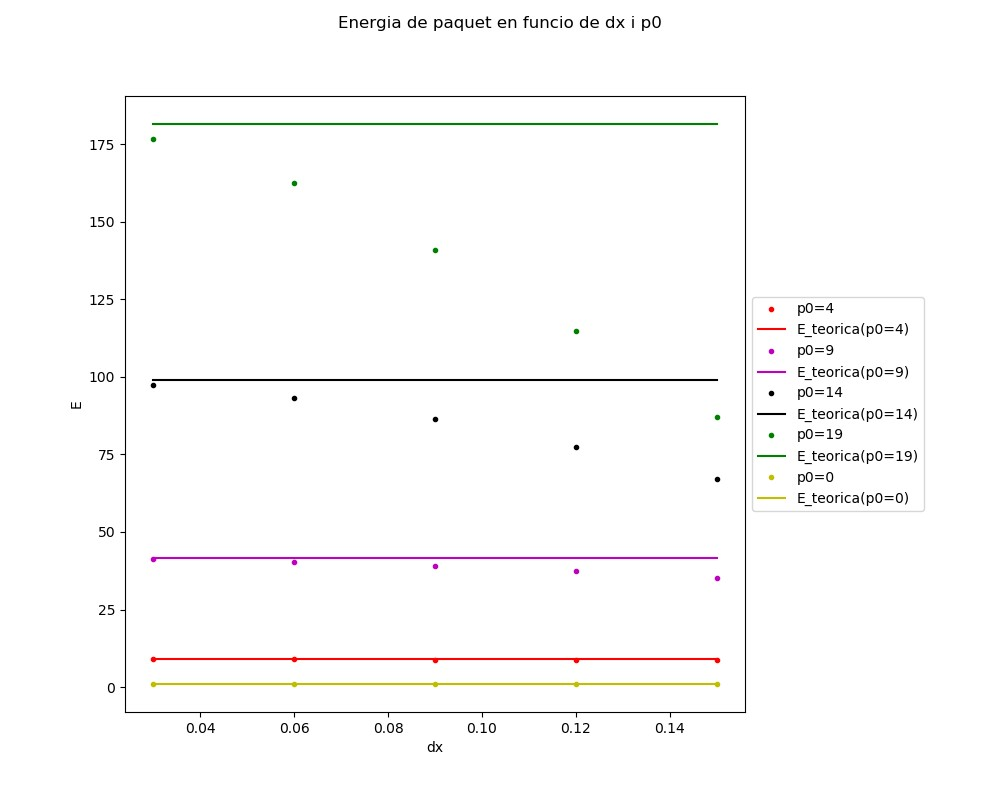
\includegraphics[width=\textwidth,height=15cm]{problemaenergia6.jpg}
	\caption{Energia cinètica de diversos paquets i la seva predicció teòrica}
\end{figure}

D'aquí podem concloure, primer de tot, que quan més moment tingui el paquet, és a dir, més energia total, més petit haurà de ser el discretzat en l'espai per descriure'l correctament. L'afirmació inversa també es certa, així que també hem de tenir en compte que quan més petit sigui el discretitzat, més s'allarga el temps de càlcul. Per un altre banda, un canvi en el dt no afecta signficativament a l'energia total, però si a altres aspectes com l'evolució del valor esperat. Fitem, doncs, aquests dos discretitzats:

\begin{equation}
dx<0.05, \quad dt<0.01
\end{equation}

I en quant els moments:

\begin{equation}
p<10
\end{equation}

Treballarem amb paquets de \(\sigma^2=0.25\), ja que mantenen la forma força bé.

\subsection{Evolució d'un paquet gaussià}

Fins ara no haviem aplicat encara el mètode ADI. Ara ens disposem a fer-ho. Hi ha diversos indicadors que ens poden ajudar a saber si el mètode està funcionant realment. La conservació de la norma és un d'ells, força testejada ja a l'hora de desenvolupar el mètode. Tot hi així, està bé comprovar de tant en tant si es conserva. L'altre és la conservació de la energia. Ja que tot el paquet està confinat en la caixa i res d'ell s'escapa, es pot predir que la energia del paquet es conserva. La evolució del valor esperat és, també, un altre bon indicador, ja que aquest hauria d'evolucionar anàlogament al de una partícula de la mateixa massa rebotant de paret a paret en la caixa.

\subsubsection{Conservació de la energia}

Utiltzant el paquet escollit a la secció anterior, el fem evolucionar sense cap energia potencial:

\begin{figure}[H]
	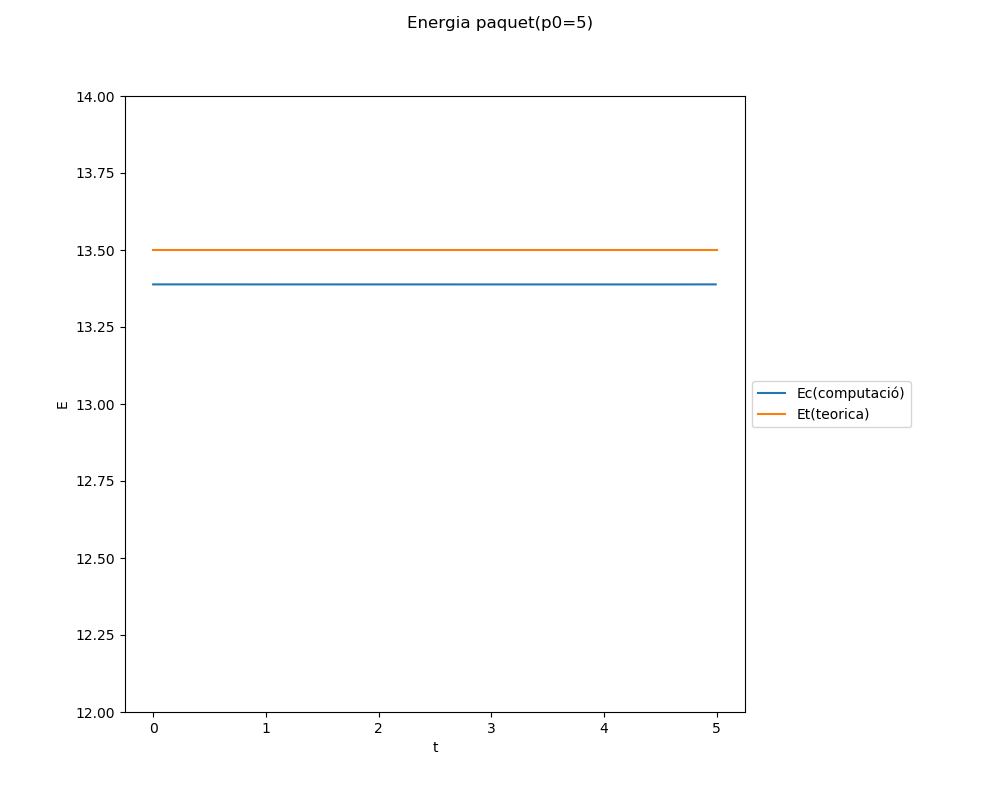
\includegraphics[width=\textwidth,height=7cm]{Ep05.png}
	\caption{Energia cinètica de un paquet de \(p_{ox}=5,p_{oy}=0\) i la seva predicció teòrica. Observem que la energia es conserva perfectament. }
\end{figure}
\begin{figure}[H]
	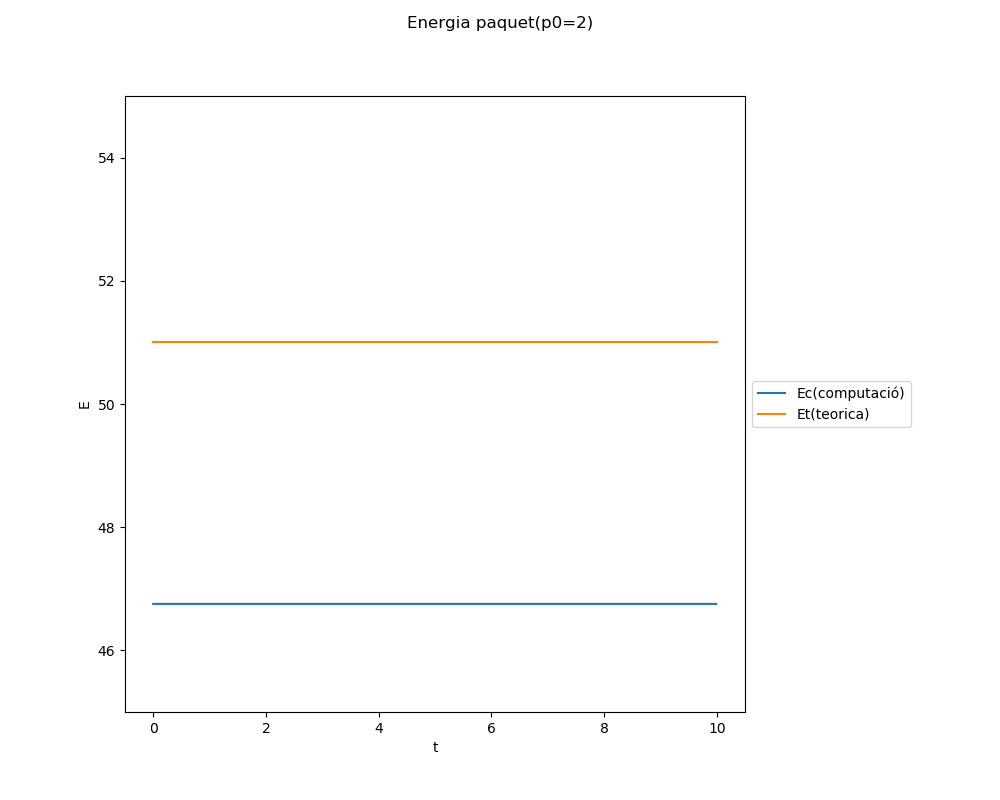
\includegraphics[width=\textwidth,height=7cm]{Ep010.png}
	\caption{Energia cinètica de un paquet de \(p_{ox}=10,p_{oy}=0\) i la seva predicció teòrica. Observem que la energia es conserva força be, tot i que hi ha una diferència força gran entre la energia teòrica i la computada. Això es degüt a l'alta energia aquí en joc. }
\end{figure}

Per tant, podem concluir que el mètode conserva força bé l'energia.

\subsubsection{Evolució del valor esperat}

Segons el Teorem d'Ethern, la evolució del valor esperat de les magnituds quàntiques d'un sistema harian d'evolucionar segons evolucionaran les clàssiques. En el nostre cas, això es tradueix en que el valor esperat en x del paquet hauria de tenir el mateix valor que una partícula de la mateixa massa dins la mateixa caixa amb la mateixa velocitat. Per tant:

\begin{equation}
v=\frac{p}{m}, \quad <X>=vt 
\end{equation}

En el primer intent, vam obtenir una cosa com aquesta:

\begin{figure}[H]
	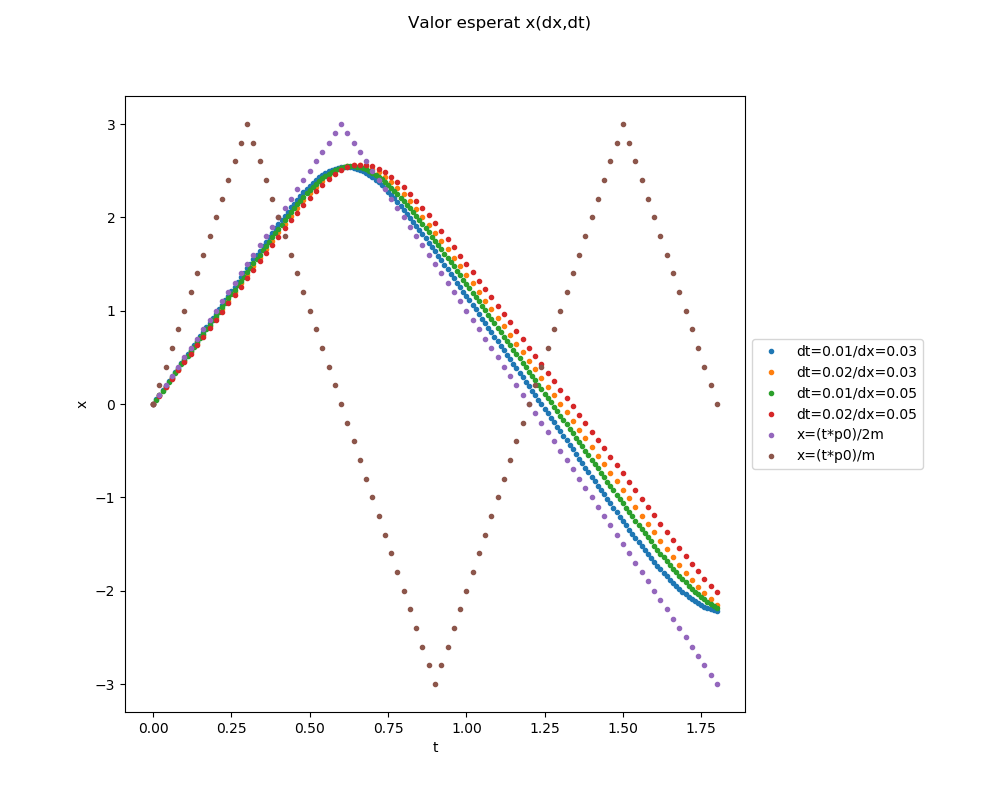
\includegraphics[width=\textwidth,height=7cm]{xespxmalament.png}
	\caption{Valor esperat del paquet i la seva predicció}
\end{figure}

El problema que generava aquest desajustament era bastant greu i solucionar-ho em va prendre molt temps.

Un cop solucionat, i utilitzant aquelles prediccions obtenim les següents figures:

\begin{figure}[H]
	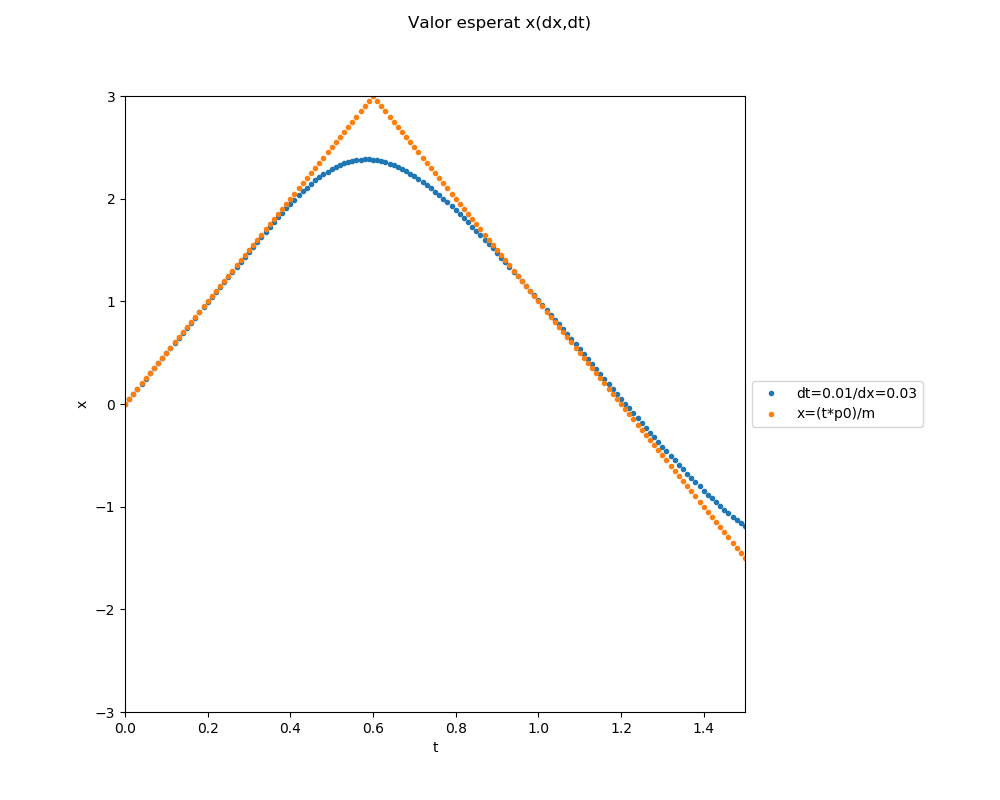
\includegraphics[width=\textwidth,height=7cm]{xespxp05dt0.png}
	\caption{Valor esperat del paquet de \(p_{ox}=5,p_{oy}=0\) i la seva predicció teòrica. Observem que coincideix bé el valor esperat teòric amb el calculat. }
\end{figure}
\begin{figure}[H]
	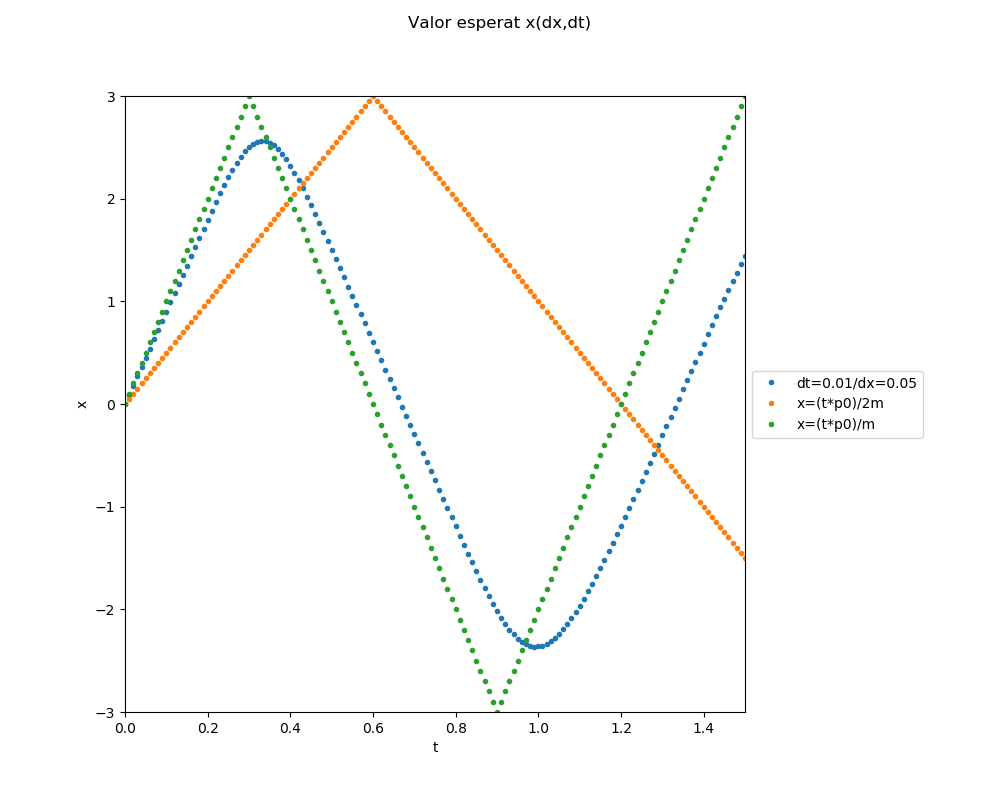
\includegraphics[width=\textwidth,height=7cm]{xespxp010dt0.png}
	\caption{ Valor esperat del paquet de \(p_{ox}=10,p_{oy}=0\) i la seva predicció teòrica. Observem que el valor esperat teòric no coincideix tan bé amb el calculat. Això és degüt a la diferència major entre energia computada i teòrica de un paquet amb aquest moment més alt, que en aquest cas és menor.}
\end{figure}

Així, podem afirmar que el nostre mètode ADI està describint correctament la evolució del moment esperat del paquet, tot i que el moment s'ha de mantenir petit. 

\subsubsection{Evolució de la dispersió en x}

Per un paquet gaussia que evoluciona lliurament, podem descriure la seva evolució en el temps així:

\begin{equation}
\sigma_x^2(t)=\sigma_x^2(0)+\frac{\sigma_p^2}{m^2}t^2, \quad \sigma_p^2=\frac{\hbar^2}{4\sigma_x^2}
\end{equation}

Tot i que sabem que aquesta evolució correspón a la de un paquet que és lliure, tenim que inicialment la \(\sigma_x^2\) computada ha de coincidir amb la teorica. Per tant, podem utiltizar aquesta equació per predir les diespersions del paquet almenys en els temps inicials. Obtenim les següents figures:

\begin{figure}[H]
	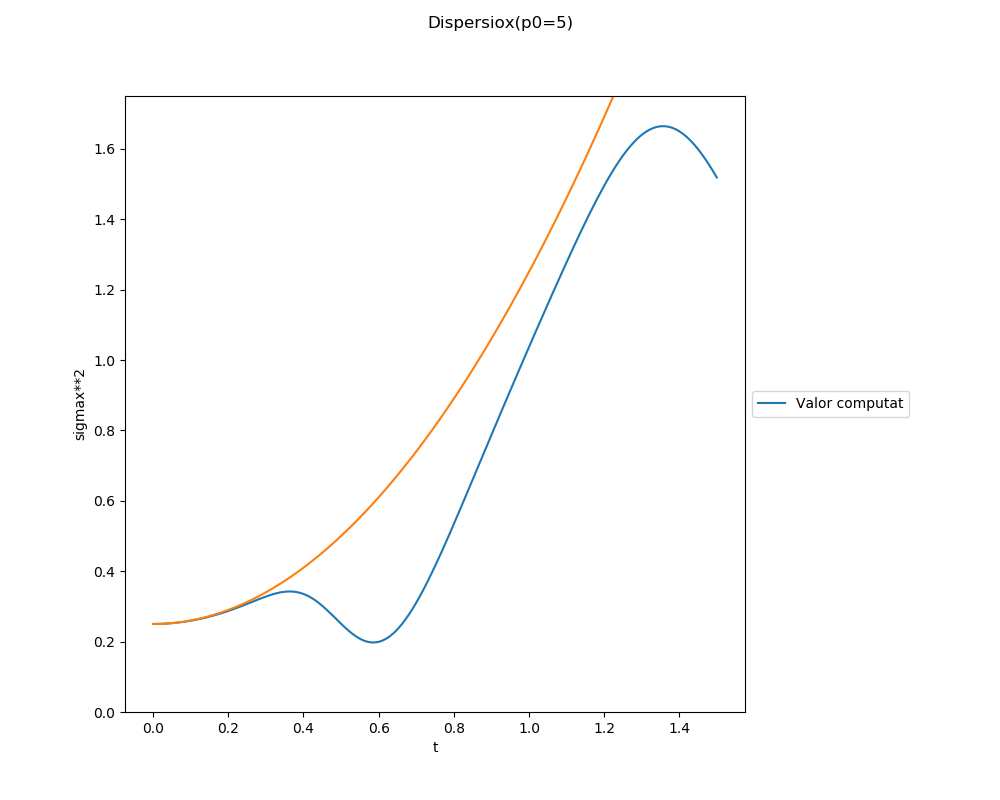
\includegraphics[width=\textwidth,height=7cm]{dispersioxpo5.png}
	\caption{Dispersio en x del paquet de \(p_{ox}=5,p_{oy}=0\) i la seva predicció teòrica. Observem que les dues funcions coincideixen bé inicialment. Posteriorment, ens trobem amb que el paquet xoca amb la paret, el que redueix repentinament la dispersió.}
\end{figure}
\begin{figure}[H]
	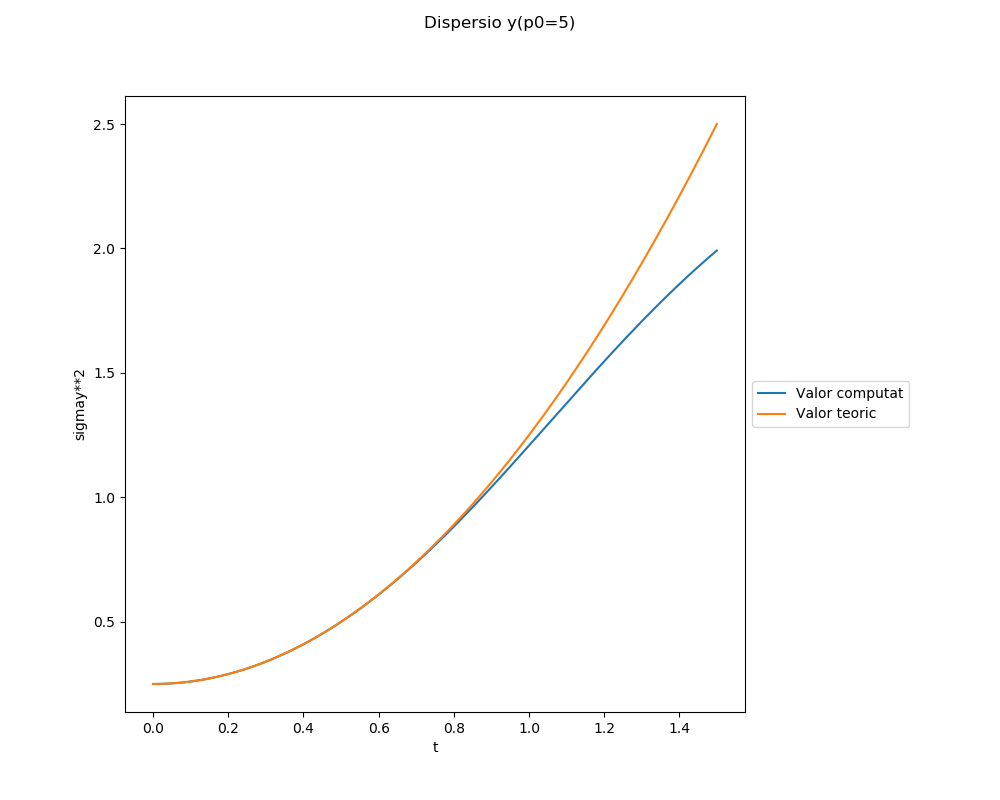
\includegraphics[width=\textwidth,height=7cm]{dispersioypo05.png}
	\caption{ Dispersio en y de \(p_{ox}=5,p_{oy}=0\) i la seva predicció teòrica. Observem que les dues funcions coincideixen bé durant un temps. Ja que no hi ha cap xoc amb les parets de \(y=\pm L\), les funcions coincideixen més temps que en la figura anterior.}
\end{figure}

El comportament de la dispersió del paquet computat coincideix amb el teòric. Per tant, la evolució de la dispersió del paquet es correcte (coincideix amb la teòrica) .

\subsubsection{Conservació de la norma}
Sense dubte, el millor indicador de que el mètode funciona és la conservació de la norma del paquet. La norma s'obte facilment, multiplicant \(\psi\)  pel seu conjugat e integrant sobre tot l'espai. Així, obtenim la següent figura:

\begin{figure}[H]
	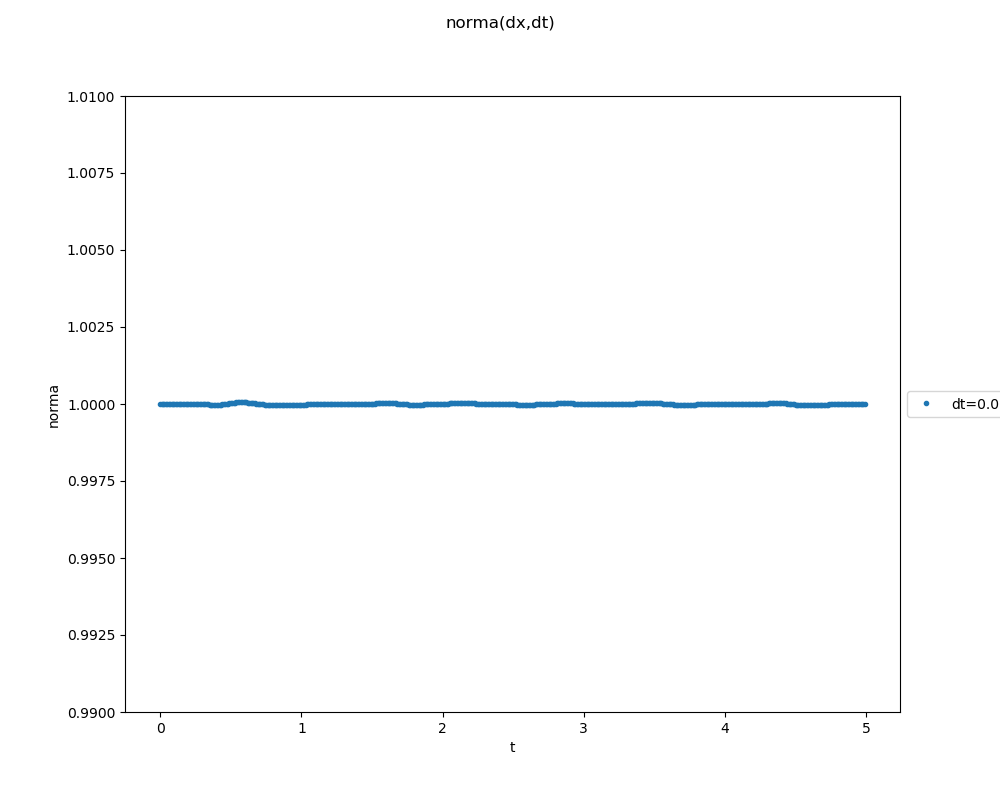
\includegraphics[width=\textwidth,height=7cm]{normadiscretizatp05.png}
	\caption{Norma del paquet de \(p_{ox}=5,p_{oy}=0\). Observem que es conserva perfectament}
\end{figure}
\subsection{Oscilador harmònic}
Un altre manera de veure si el mètode funciona es a partir de l'oscilador harmònic. Fins ara, hem fet evolucionar el paquet sense cap potencial. Observem que passa amb aquests tipus de paquets.

La solució del osiclador harmònic en 2D en MQ és analítica. Això vol dir que per un donat potencial quadràtic harmònic puc coneixer tant els seus autoestats
com el valor que haurà de prendre tant l'energia cinètica com la potencial, i per tant, la total. Puc utilitzar aqueset fet per comporvar si el meu codi
descriu correctament l'evolució d'aquests autoestats, i també si estic efectuant, de manera correcta, el càlcul de la energia. 


El primer que farem es avaluar independentment el càlcul de la energia a partir de estats fonamentals inicials (sense fer-los evolucionar amb el mètode). Tot següit, i un cop aquesta descripció sigui correcta, evolucuionarem diversos estats fonamentals i comporvarem si verifiquen la solució
analítica.

\subsubsection{Descripció física}
Considerem un Hamiltonia tal que:
\begin{equation}
H=\frac{P^2}{2m}+\frac{1}{2}m\omega^2(X^2+Y^2)
\end{equation}

on \(P^2=(-i\hbar\nabla)^2=- (\frac{\partial^2}{\partial x^2}+\frac{\partial^2}{\partial y^2}) \). Hesisenberg va solucion analíticament aquest problema en 1 dimensió. En el nostre cas, el problema es pot resoldre independentment per cada dimensió i després simplement combinar les dues solucions (això ho podem fer perquè \(H=H_x+H_y\)).

Els autovalors de H seràn, llavors:

\begin{equation}
E_{n_x,n_y}=\hbar\omega(n_x+n_y +1 ), \quad n_x,n_y=0,1,2,3...
\end{equation}

I tenint en compte que \(<X^2>,<Y^2>=\frac{\hbar}{m\omega}(n+ \frac{1}{2})\) i que \(<P_x^2>,<P_y^2>=m\hbar\omega(n+ \frac{1}{2})\), tenim per les energias cinètiques i potencial:
\begin{equation}
Ec_{n_x,n_y}=\frac{\hbar\omega}{2}(n_x+n_y+1)
\end{equation}
\begin{equation}
Ep_{n_x,n_y}=\frac{\hbar\omega}{2}(n_x+n_y+1)
\end{equation}

Per un altre banda, els autovectors corresponents a cada un dels autovalors seràn:
\begin{equation}
\phi_{n_x,n_y}(x,y)=\sqrt{\frac{1}{2^{n_x+n_y}n_x!n_y!b^2\pi}}H_{n_x}(x/b)H_{n_y}(y/b)e^{-\frac{1}{2b^2}(x^2 +y^2)}
\end{equation}

on \(b=\sqrt{\frac{\hbar}{m\omega}}\)

\subsubsection{Aplicació}
Per testificar el nostre  codi, només ens caldra testejar un autoestat. Escollirem el més senzill, per tant el fonamental. És a dir, \(n_x=0,n_y=0\).
La idea és que donats diversos potencials harmònics amb diversos valors de la w, calcular pels seu autoestat fonamental corresponent el valor de la Ec
i Ep, tant com el valor esperat de X i Y. Diveross w implican diversas energias, per tant, podrem traballar en un ampli abanic d'energias diferents 
per així observar si la solució computada s'allunya de la analítica en funció de la energia.

Per tant, utilitzarem un paquet tal que:
\begin{equation}
\phi_w(x,y)=\sqrt{\frac{\omega m}{\hbar\pi}}e^{-\frac{m\omega}{2\hbar}(x^2 +y^2)}
\end{equation}

I un potencial així:
\begin{equation}
V_w=\frac{1}{2}m\omega^2(X^2+Y^2)
\end{equation}

Per tant, la seva energia serà:

\begin{equation}
E=\hbar\omega, \quad E_c=\frac{\hbar\omega}{2}, \quad E_p=\frac{\hbar\omega}{2}
\end{equation}

\subsubsection{Paquet sense evolució}
En aquest apartat, únicament crearem diversos estats i els discretizarem amb el mateix criteri que seguim a l'hora de crear-los per introduir-los a l'algoritme de Crank-Nicolson. Tot seguït, calcularem la seva energia cinètica i potencial i observarem si ha discrepàncies amb el que prediu la teoria. Farem el mateix pels valors esperats.

Els valors de omega escollits aniran, més o menys, de valors que faguin \(E<150\), ja que més enlla el discretitzat ha des ser cada cop més petit per 
aconseguir una descripció correcta. Per tant, ecollirem un \(dx=0.03\) i un rang de \(\omega=15n\) per \(n=1,2,..,10\). Introduïrem l'autoestat a una caixa quadrada de a=2L=6 ja que és aquí on el desenvolupament del joc té lloc. Ja que els càlculs analítics es fan considerant un espai infinit, aquest fet
farà que sigui imposible que coincideixin exàctament els dos valors de la energia. No obstant, l'aproximació de considerar que el paquet es trobaba en un espai infinita i no en una caixa ha funcionat prou bé en càlculs analítcs anteriors, per tant, la tornem a aplicar sense previsiblement cap problema.

Un cop calculada, utlitzant la funció utiltizada anteriorment, tenim que:

\begin{figure}[H]
	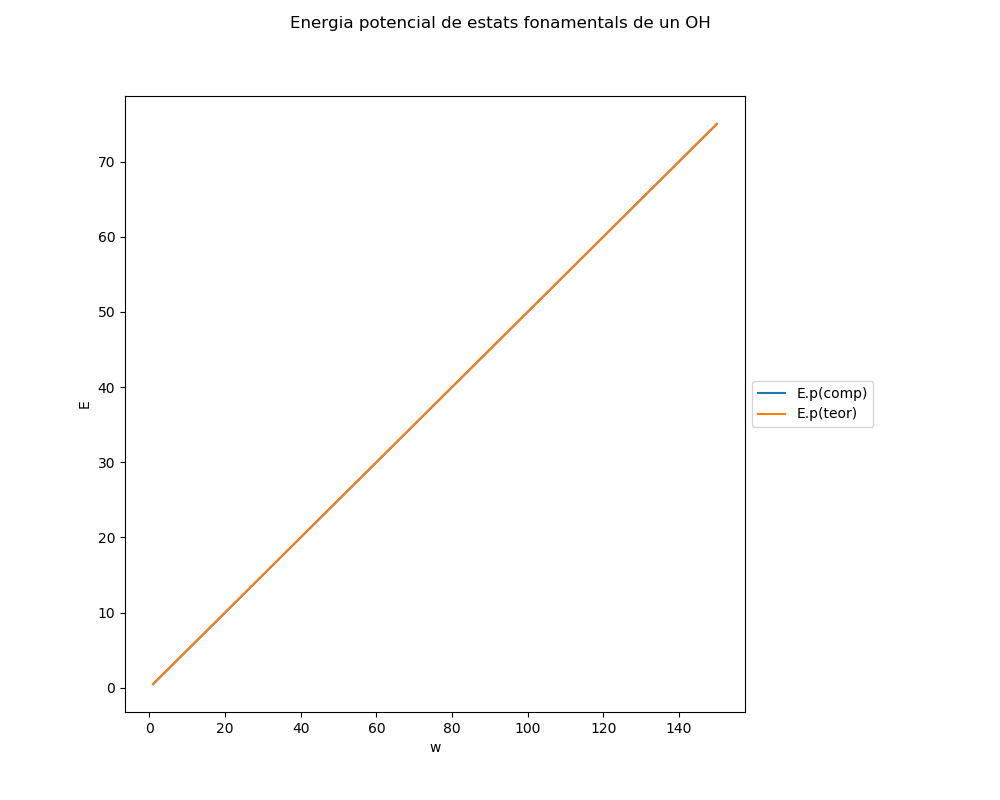
\includegraphics[width=\textwidth]{Epotharm.png}
\end{figure}
\begin{figure}[H]
	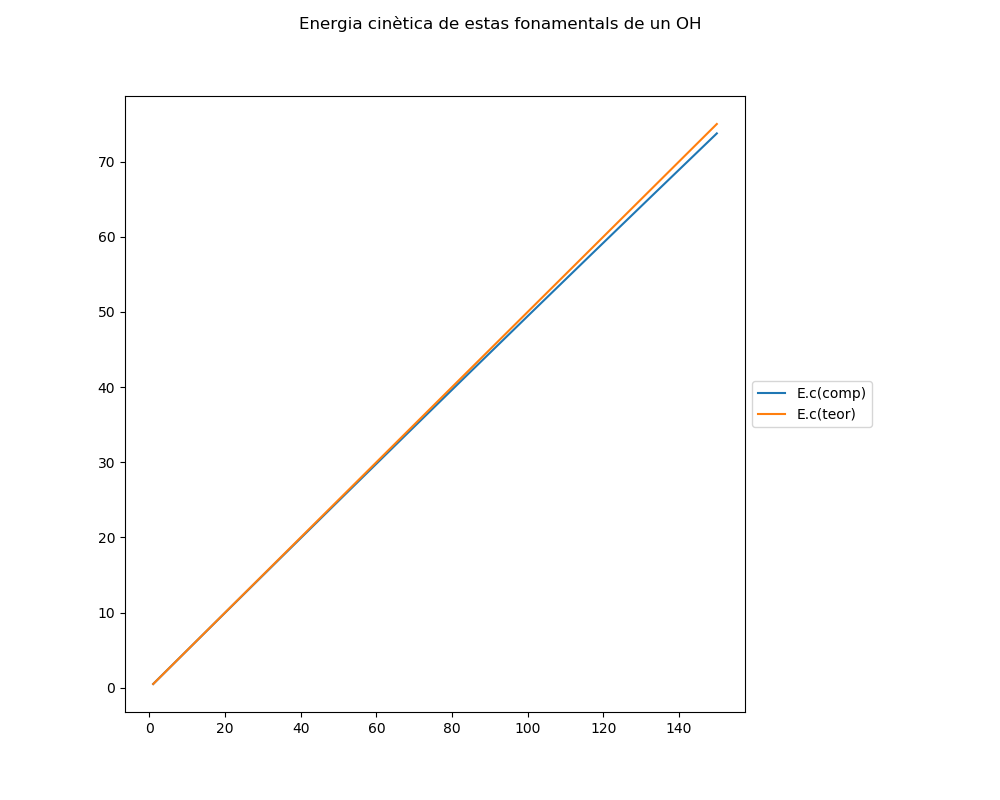
\includegraphics[width=\textwidth]{Ecinharm.png}
	\caption{Energia cinètica i potèncial de l'estat fonamental (\(n_x=0,n_y=0\)) de diversos oscil·ladors harmònic}
\end{figure}

A partir de la Figura 1, s'observa que el procediment per calcular la energia cinètica i potèncial dels paquets discretitzats és correcte i per tant,
no seran una font d'error a l'hora de procedir amb el càlcul de la energia durant l'evolució dels paquets. Per un altre banda, hem obtingut un procediment
per comparar amb càlculs analítics els càlculs propis de la energia cinètica i potencial. És a dir, un procediment per saber en tot moment si el paquet 
està evolucionant correctament. 

\subsubsection{Evolució de l'estat}

Fins ara, estavem únicament considerant l'estat fonamental inicial. No obstant, el que volem testejar
realment es quin efecte té la evolució de l'estat pel mètode de Crank-Nicolson construït en els paràmetres inicials d'aquests. El millor indicador de que el mètode funciona és que l'energia total es conserva. En aquest cas, a partir de (8), hauríem de esperar inclús la conservació de la energia cinètica i potencial durant tot temps d'evolució. Un altre bon indicador de que el mètode es coherent físicament és comporbar que el valor esperar de X e Y és manté en 0, que és el que cal esperar. 

Així doncs, aplicarem l'evolució de Crank-Nicolson durant un cert temps, \(t\). Tenint en compte el temps de càlcul necessàri, ens decantarem per fer aquest \(t=1\), ja que ja ens es suficient per observar si el mètode divergeix o no. En un principi, escollirem un \(w=50\).

Finalment, obtenim això:

\begin{figure}[H]
	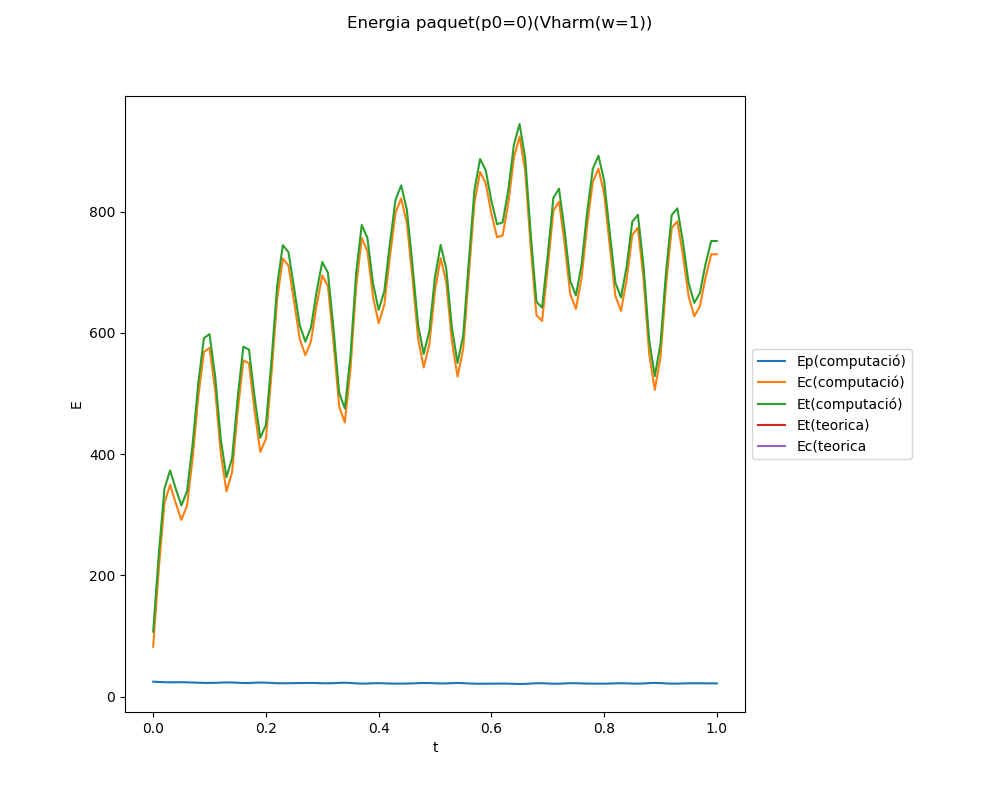
\includegraphics[width=\textwidth]{energiaharmdiscretitzat.png}
	\caption{Energia cinètica i potèncial de l'estat fonamental (\(n_x=0,n_y=0\)) de l'oscilador w=50 en diversos instants de t}
\end{figure}

Aquesta figura ens indica que alguna cosa no està funcionant correctament. La manera de calcular la energia cinètica i potencial per un instant t s'ha demostrat que és correcte. Per un altre banda, el càlcul de la energia en funció del temps ja s'ha fet anteriorment utilitzant just el mateix mètode. Per això, no dubtem que la font del problema no és el càlcul de la energia, i opinem que es el propi codi, el propi mètode CK2D. En la figura i en els càlculs, s'observa que la energia potèncial calculada és més o menys correcte:

\begin{figure}[H]
	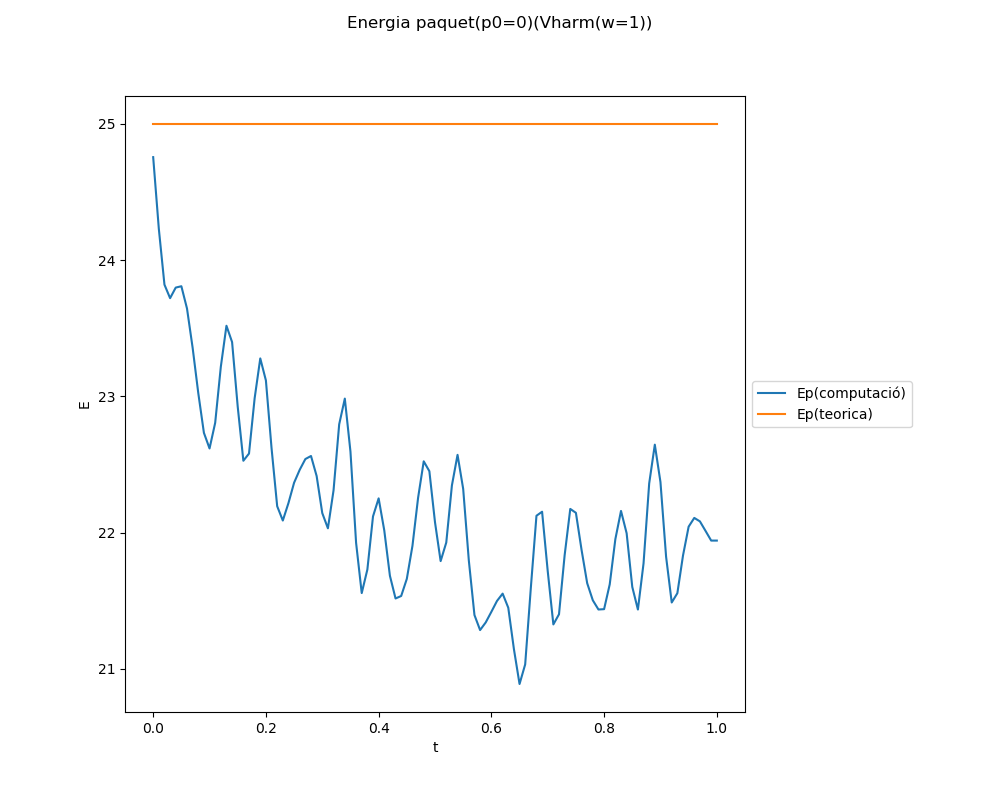
\includegraphics[width=\textwidth]{energiaharmdiscretitzatpot.png}
	\caption{Energia potèncial de l'estat fonamental (\(n_x=0,n_y=0\)) de l'oscilador w=50 en diversos instants de t}
\end{figure}

Aquesta figura no està ni molt menys bé, però es una consecuència de la conservació de la norma. Ja que quan calculem la energia potencial estem, de fet, calculant una suma \(norma[i,j]V[i,j]\), ens trobem que el valor de la energia potencial no s'allunya tant del correcte. La energia cinètica, en canvi, es calcula amb la derivada segona de \(phi\) i per tant, que aquest paràmetre es dispari tant ens fa pensar que hi ha grans diferències en els valors de \(phi\). Per tant, l'error porbablement prove del codi. Així doncs, el revisarem i de pas, descriurem una mica el procediment que utilitzem per descriure'l.

Finalment, tras un llarg estudi del codi, ens hem adonat d'un error en l'aplicació del mètode. Un cop canviat, depurat i provat, tenim la següent figura:

\begin{figure}[H]
	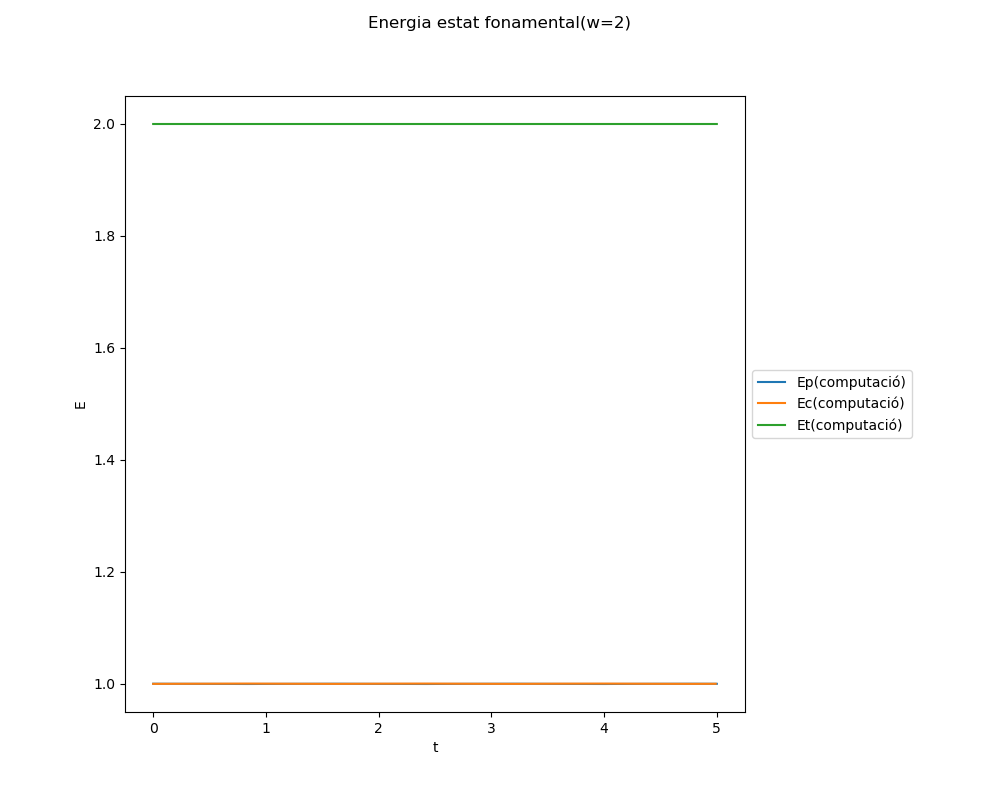
\includegraphics[width=\textwidth,height=8cm]{Eharm2.png}
	\caption{Energia potèncial de l'estat fonamental (\(n_x=0,n_y=0\)) de l'oscilador w=2 en diversos instants de t}
\end{figure}
\begin{figure}[H]
	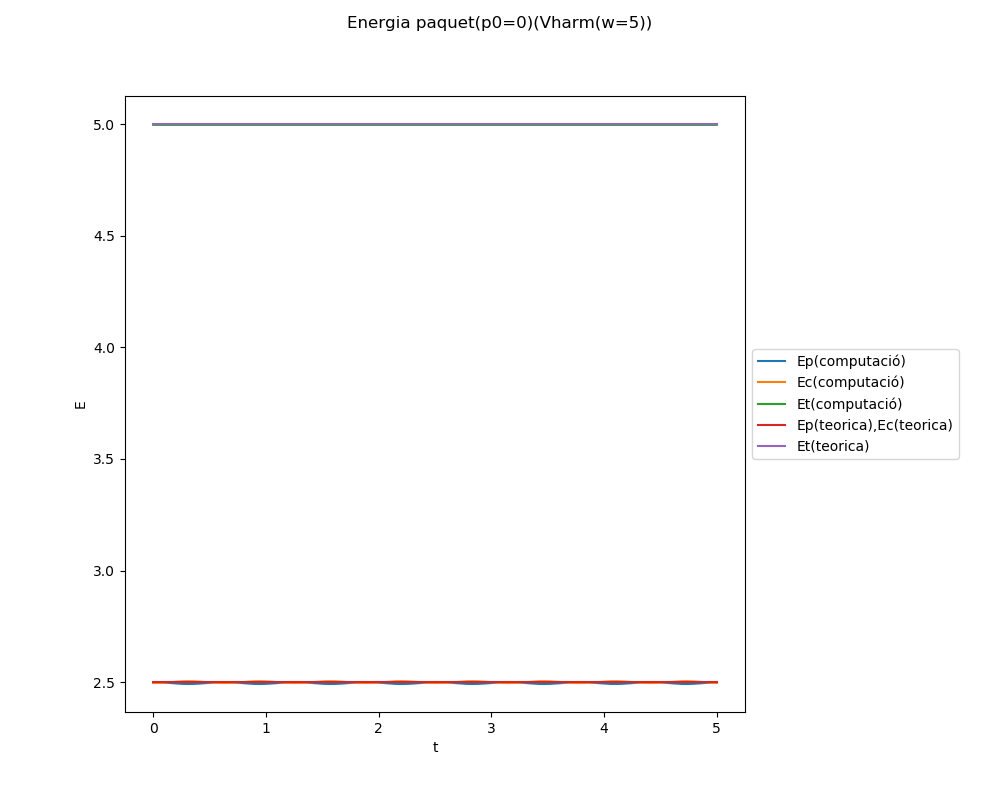
\includegraphics[width=\textwidth,height=8cm]{Eharmpot3.png}
	\caption{Energia potèncial de l'estat fonamental (\(n_x=0,n_y=0\)) de l'oscilador w=5 en diversos instants de t}
\end{figure}
\begin{figure}[H]
	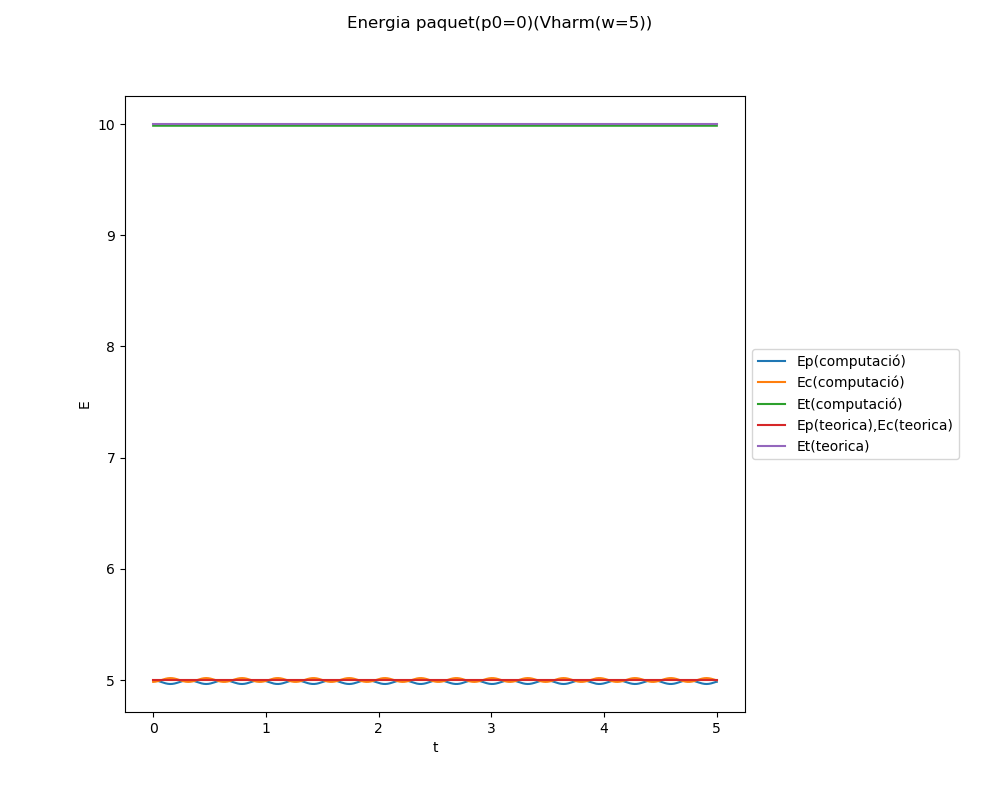
\includegraphics[width=\textwidth,height=8cm]{Eharmpot4.png}
	\caption{Energia potèncial de l'estat fonamental (\(n_x=0,n_y=0\)) de l'oscilador w=10 en diversos instants de t}
\end{figure}

Podem observar unes petites oscil·lacions en la energia cinètica i potencial. No obstant, la energia total és correcta. No sabem bé a que es deuen aquestes oscilacions. Sembla ser que segons augmentem la energia, augmentem el seu periode. Tot i així la energia total és manté constant en general, i la energia cinètica i potencial tambe són més o menys constants. 
\end{document}


\begin{thebibliography}{56}
\bibitem{pythonturial}
\textit{The python tutorial}
https://docs.python.org/3/tutorial/
https://la-mecanica-cuantica.blogspot.com/2009/08/estados-coherentes.html
\end{thebibliography}


